\chapter{Effect of Operating Systems on Results}

In this chapter, we present an observation made while evaluating our proposed
scheduler, namely the simulation results varied depending on which operating
system the simulation was run. In Sec.~\ref{sec:effect} the effect of our
observation on measured performance metrics is shown. The result of conducted
numerical experiments to investigate possible reasons for different OS behavior
is given in Sec.~\ref{sec:experiments}

\section{Overview} \label{sec:effect}

All simulations for this thesis were performed on a NCS software framework
implemented in C++\footnotemark. During the course of evaluation, we have
discovered numerical inconsistencies in measured network average
$\overline{MSE}$ and AoI $\overline{\Delta}$ among simulations performed on
Linux, Mac and Windows platforms. For reproducibility, Tab.~(\ref{tab:specs})
lists specification for the used computing systems. It should be pointed out
that FHS and GES evaluations were performed under Linux, while simulation on Mac
and Windows were conducted for investigation purposes.

\begin{table}[b]
  \begin{center}
  \begin{tabular}{|l|c|c|c|} 
  % \begin{tabular}{|l|c|c|>{\centering\arraybackslash}p{3.4cm}|} 
  \hline
  \textbf{Environment} & \textbf{Linux} & \textbf{Mac} & \textbf{Windows} \\
  \hline \hline
  Compiler & g++ 8.4.0 & Apple clang 11.0.0 & g++ 10.2.0 (Mingw-w64) \\ 
  Operating System & Ubuntu 18.04.05 & macOS 10.15.7 & Windows 10 Ver. 1809 \\ 
  % Kernel & GNU/Linux 4.15.0-117-generic x86\_64 & x86\_64-apple-darwin19.6.0 & WIN32 \\ 
  CPU & 0.3 & Intel Core i5-4260U & Intel Core i5-4670 \\
  % Cores & 32 & 4 & 4 \\
  \hline
  \end{tabular}
  \end{center}
  \caption[Summary of runtime environment for tested simulation
  platforms]{Summary of runtime environment for tested simulation platforms.
  Note that Mingw-64 is a port of the GNU Compiler Collection (GCC) for
  Windows.}
  \label{tab:specs}
\end{table}

To make the investigation more tractable, we replace the GE model with a simpler
channel model. As reference case, the setting from \cite{ayan2020aoi} is taken,
which utilizes the base FH scheduler. Here, $N=3$ heterogenous NCSs with system
matrices $A_i\in\left\{1.0, 1.25, 1.5 \right\}$ share a lossy wireless channel
with i.i.d normal packet loss, i.e., $p_i(t) \sim \mathcal{N}(0.3,0.2)$. 

Fig.~(\ref{fig:observation}) illustrates our findings for measured
$\overline{MSE}$ and $\overline{\Delta}$ vs. finite horizon $H=\left\{1, \dots,
9\right\}$ over 200 simulation runs. We can examine the same decreasing trend
for both metrics on all OSs. However the absolute deviations are quite
significant. In particular, the estimation error at Horizon $H=1$ deviate
between Windows and Linux for almost 50\%. This effect is not negligible, since
our proposed scheduler uses expected MSE to form scheduling decisions. On the
the hand, between Mac and Linux a minor but consistent difference is observed
for both metrics. In contrast, for $\overline{MSE}$, the Windows trajectory
starts following the Mac trajectory until $H=5$, where it coincides with Linux
values. In case of network average AoI $\overline{\Delta}$, the Windows
trajectory does not follow a specific OS but rather progresses individually.

\begin{figure}[htb]
  \centering
  \begin{subfigure}[b]{0.49\textwidth}
    \centering
    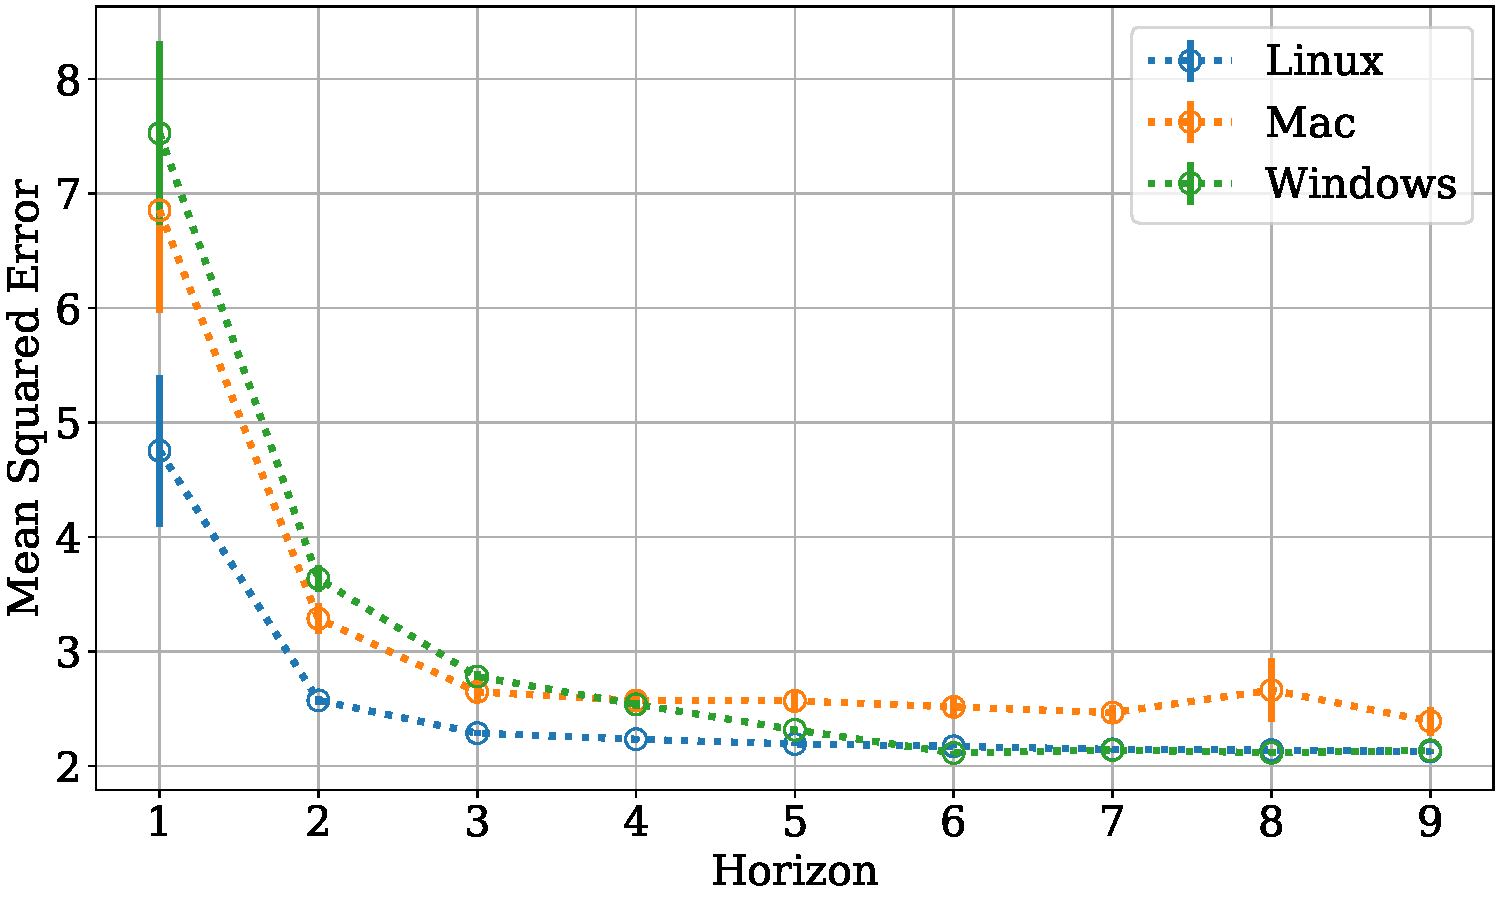
\includegraphics[width=\textwidth]{OS_MSE_against_H} 
    \caption{Network average estimation error $\overline{MSE}$}
    \label{fig:osmse}
  \end{subfigure}
  \hfill
  \begin{subfigure}[b]{0.49\textwidth}
    \centering
    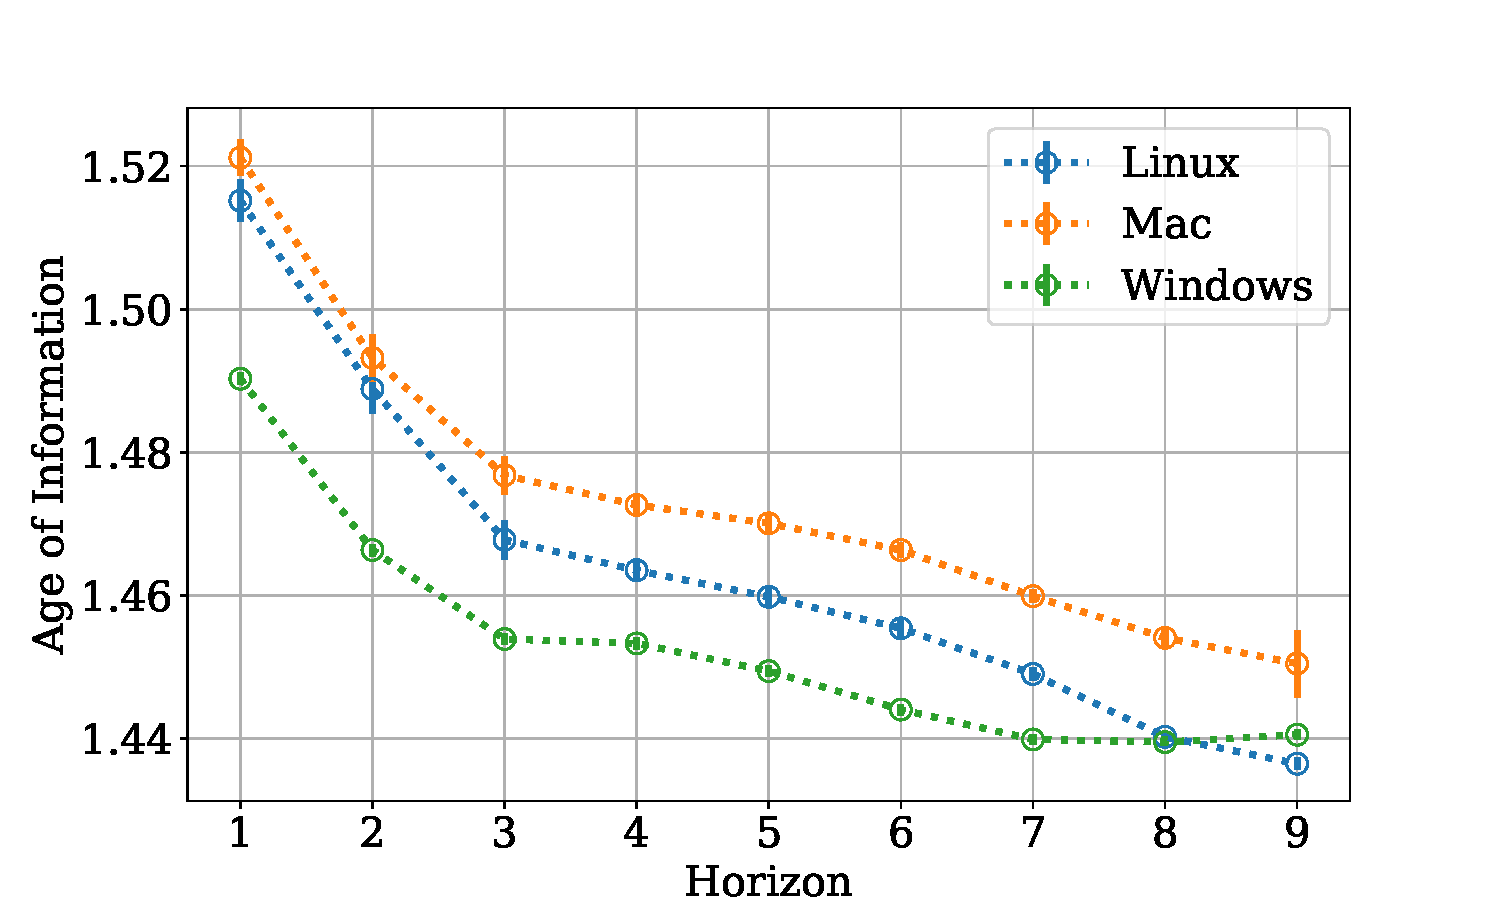
\includegraphics[width=\textwidth]{OS_AoI_against_H} 
    \caption{Network average AoI $\overline{\Delta}$}
  \end{subfigure}
  \caption[Comparison of network average MSE and AoI for different OS]{The two
  plots show $\overline{MSE}$ and $\overline{\Delta}$ for 200 simulation
  repetitions on Linux, Mac and Windows. Vertical error bars represent 95\%
  confidence intervals.}
  \label{fig:observation}
\end{figure}

Possible reasons for different OS behavior can root from either the algorithm or
its runtime implementation. From the algorithm's point of view MSE, is
influenced by the quality of estimations, which are governed by information
freshness. In contrast, AoI is solely dependent on network outcome, which is
governed by the scheduling decisions made at each time slot and the packet loss
process. The outcome of packet transmission may vary between OSs if their random
number generators differ. Independent of the algorithm's design, the way it is
executed on a computing environment relies on the specific compiler. That is,
the compiler translates our simulation code into corresponding machine
instructions which can be run on the underlying hardware. Different
implementations on an lower level can also produce numerical inaccuracies
affecting algorithm behavior. Note that a thorough analysis on these lower
abstraction levels are beyond the scope of this thesis.

\footnotetext{The source code is available at \url{https://github.com/oayan/finite_horizon_scheduling}}

\section{Numerical Experimentation} \label{sec:experiments}

Taking aforementioned relationships into account, we suspect varying randomness
and/or numerical deviations causing inconsistent scheduling policies, to be the
reason behind observed $\overline{MSE}$ and $\overline{\Delta}$. Hence, the
following investigation focuses on these two aspects.

\subsection{Random Number Generator}

Generating random numbers on a computer forms a contradiction, as computers by
design are deterministic machines. Nevertheless, in modern computing
deterministic random bit generators are used to cope with this problem. Instead
of true random numbers, these algorithms generate ``pseudo-random'' numbers
whose properties approximate true random numbers. A prominent example is a
\textit{Mersenne Twister} generator. Pseudorandomness is caused by the initial
value, also called \textit{seed}, given to the random number generator. In
particular, the output numbers are completely determined by the seed. Therefore,
it is important to initialize random number generators with a unique seeds e.g.
hardware state information. Further, the obtained raw numbers are transformed to
a suitable distribution for desired usage.

\begin{figure}[htbp]
  \centering
  \begin{subfigure}[b]{0.49\textwidth}
      \centering
      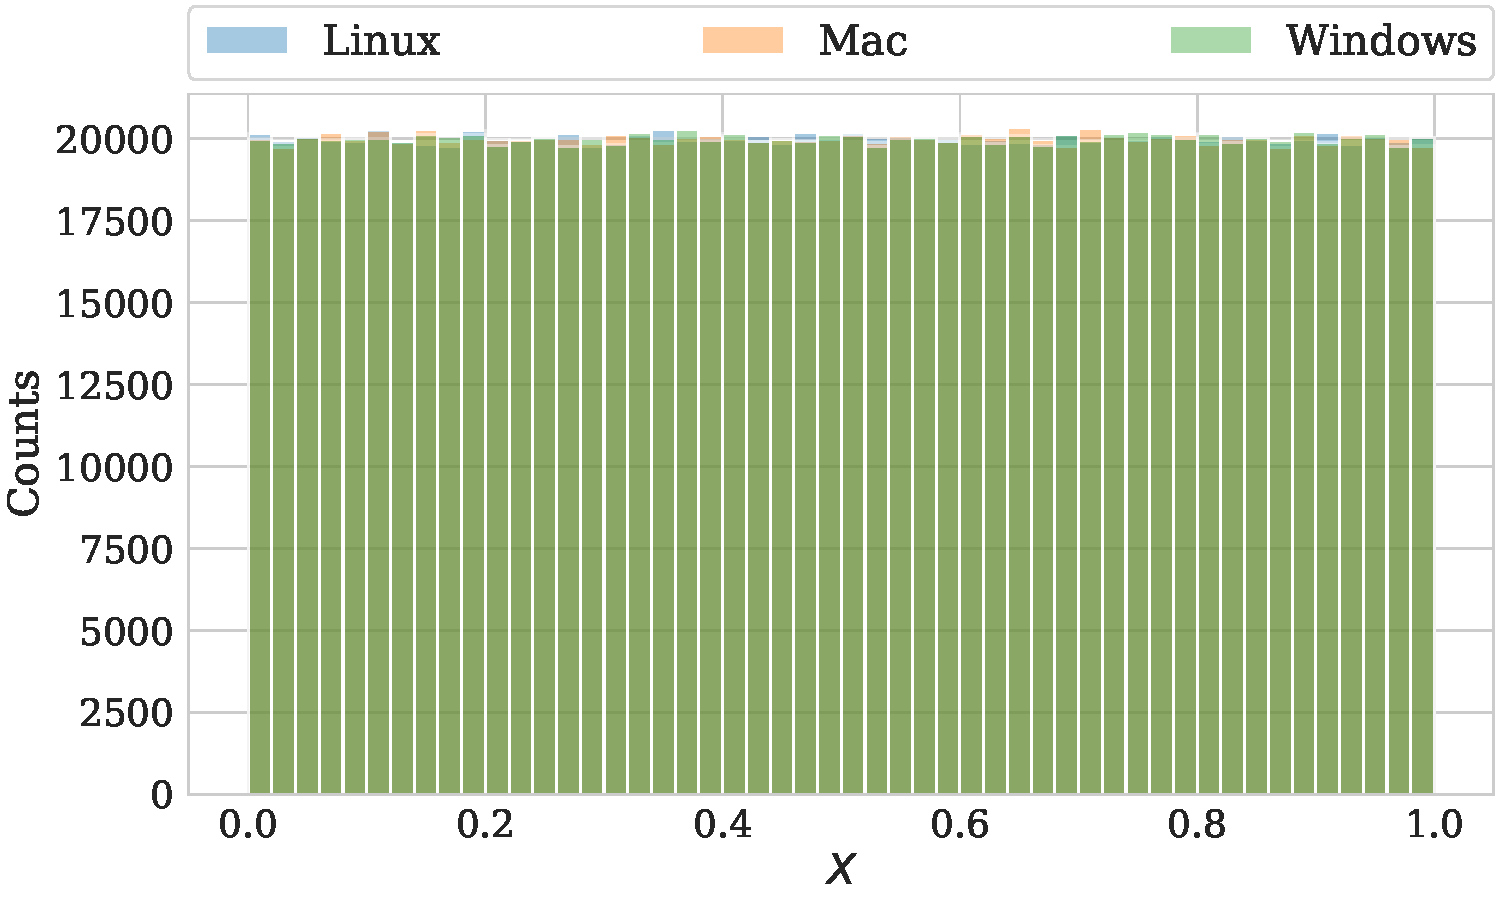
\includegraphics[width=\textwidth]{uniform}
      \caption{$X \sim \mathcal{N}(0.5, 0.2)$}
  \end{subfigure}
  \hfill
  \begin{subfigure}[b]{0.49\textwidth}
      \centering
      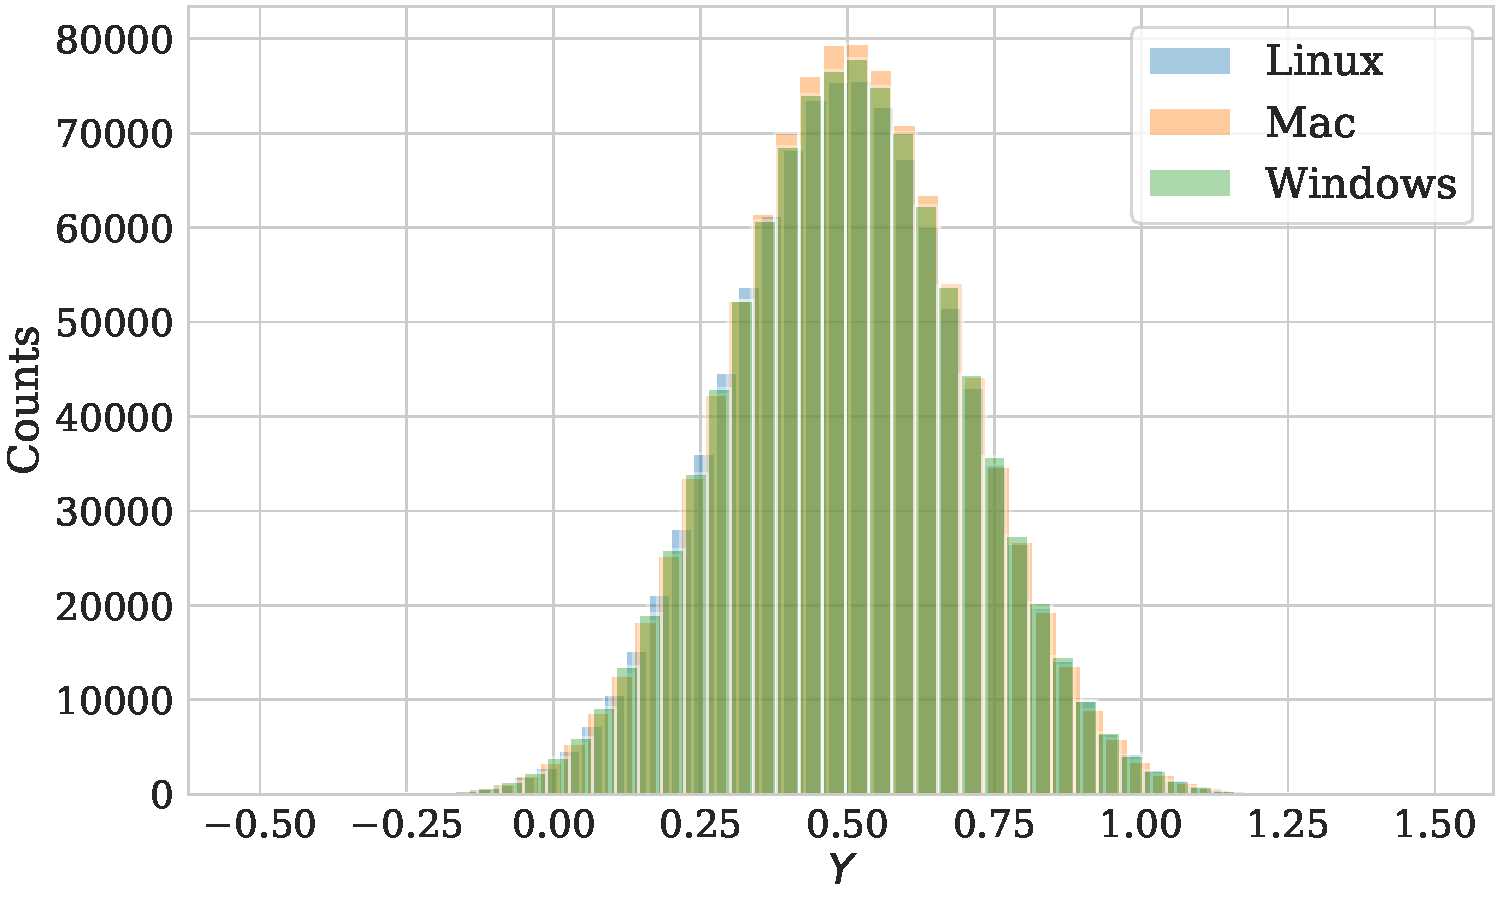
\includegraphics[width=\textwidth]{normal}
      \caption{$Y \sim \mathcal{U}(0, 1)$}
  \end{subfigure}
    \caption{The histograms of 1 million realizations of random variables utilized in simulations on Linux, Mac and Windows.}
    \label{fig:randomCheck}
\end{figure}

The used NCS simulation framework determines system noise of sub-systems and GE
channel state transitions as well as the outcome of packet transmissions from
Bernoulli experiments. The C++ standard library provides implementations for
both random engines and random number distributions. In our case, we have
deployed \texttt{std::default\_random\_engine} as random number generator, which
is seeded with the system clock count. As the simulations utilizes normal and
uniform distributions, we have generated realizations of respectively
distributed random variables $X, Y$ on all tested OSs.
Fig.~\ref{fig:randomCheck} depicts the histogram of a million realizations each.
It is visible, that the random number generator performs consistent on all three
platforms.

\subsection{Numerical effects on Scheduler}

Scheduling decisions are formed by the action which achieves minimal expected
cost as defined in Eq.~\eqref{eq:minimizationproblem}. To do so, the scheduler
is able to map measured AoI to an age-penalty following
Eq.~\eqref{eq:gfunction}. In the used NCS simulation framework, the scheduler
initializes a \textit{cost map} at each simulation run, which contains
precomputed age-penalties until a predefined maximum AoI for every simulated
sub-system. 

\begin{figure}[htbp]
  \centering
  \begin{subfigure}[b]{0.49\textwidth}
      \centering
      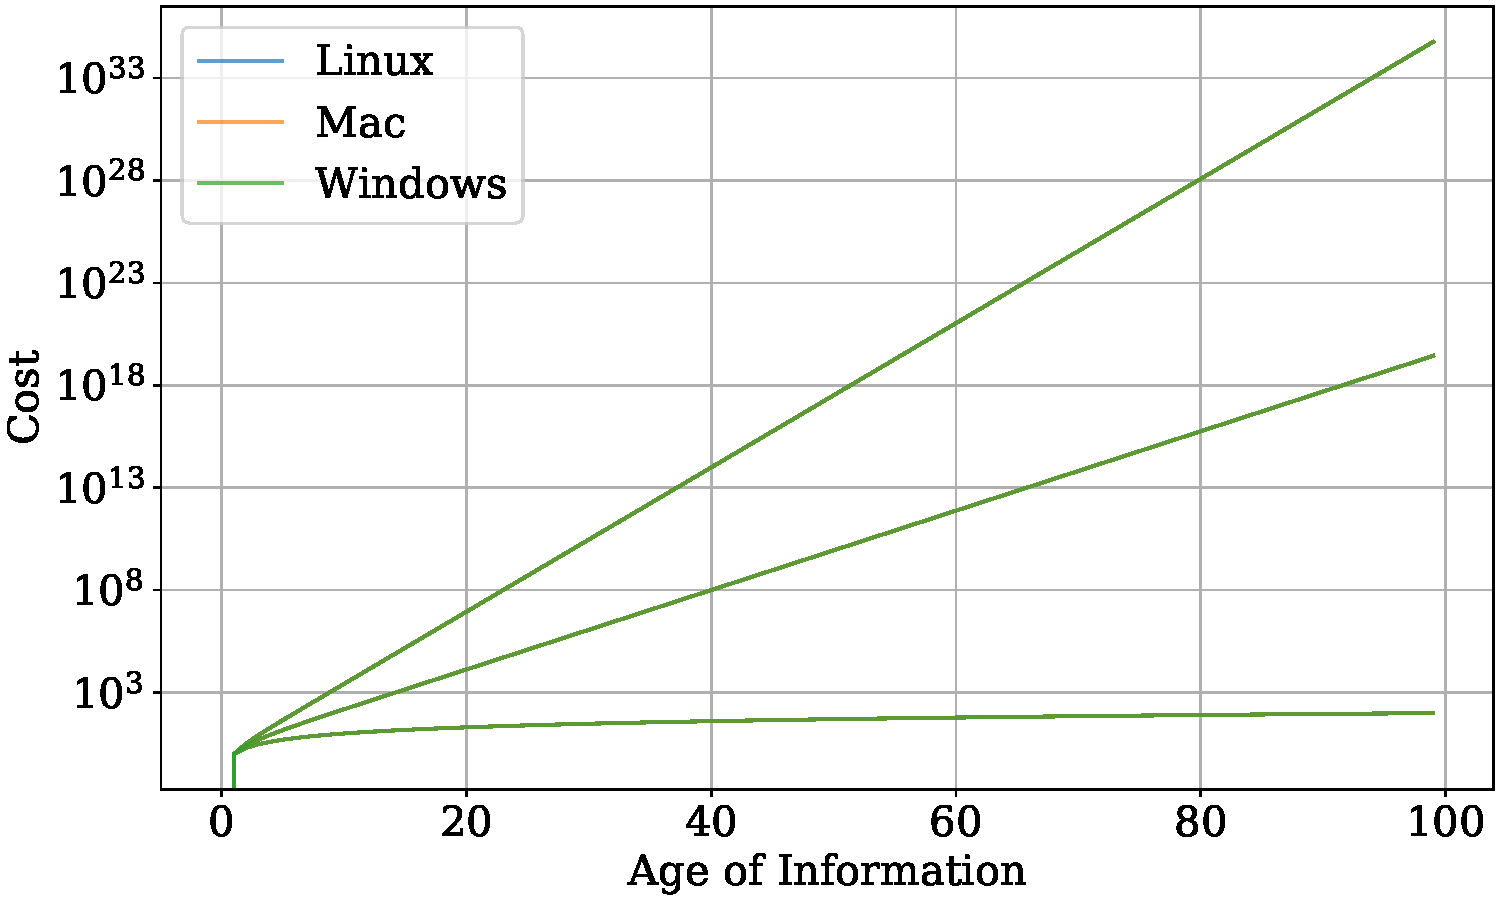
\includegraphics[width=\textwidth]{costMaps}
      \caption{Cost maps of FHS}
      \label{fig:costMaps}
  \end{subfigure}
  \hfill
  \begin{subfigure}[b]{0.49\textwidth}
      \centering
      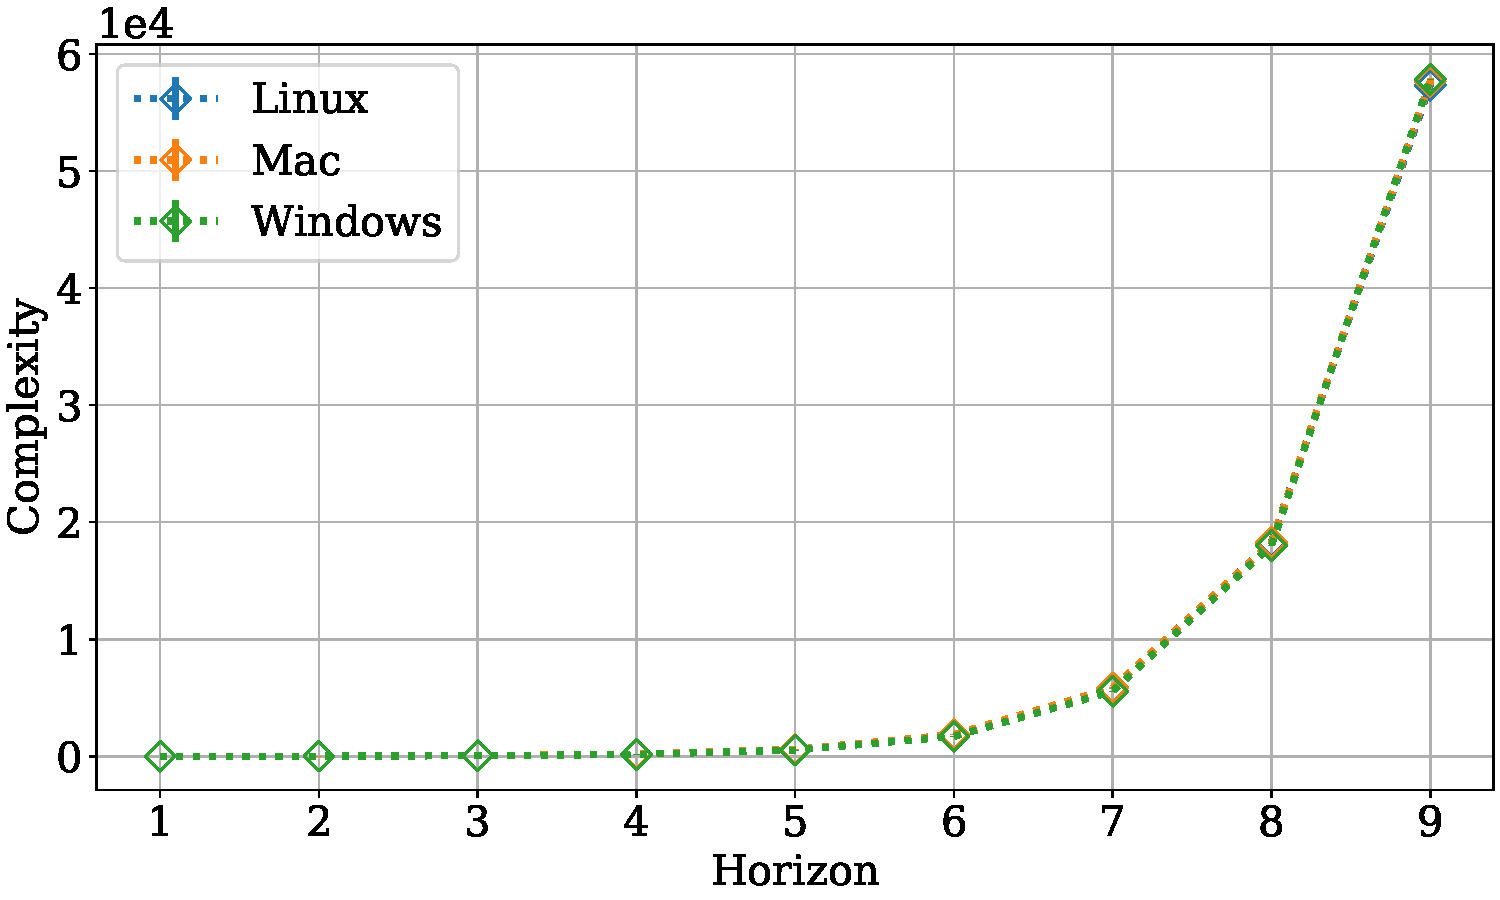
\includegraphics[width=\textwidth]{OS_AvgNodeCount_against_H}
      \caption{Average size of FHS tree}
      \label{fig:treesize}
  \end{subfigure}
    \caption[Comparison of FHS cost maps and average tree size for different
    OS]{The FHS cost maps and average tree size for Linux, Mac and Windows.}
\end{figure}

Fig.~\ref{fig:costMaps} depicts the cost maps of FHS for our considered test
scenario on different OSs. Note that, as $N=3$, a cost map consists of three
branches accounting for heterogenous control applications. We observe the same
precomputed costs among Linux, Mac and Windows. Furthermore, we have
investigated possible differences in the tree structure. The FHS employs a tree
structure to perform combinatorial optimization, which weighs possible future
nodes according to their occurrence in the tree. As seen in
Fig.~\ref{fig:treesize}, the average tree size are identical for all OSs, meaning
optimization are performed on the same tree. 

\subsection{Discussion}

The conducted numerical experimentation prove that our suspicions were wrong.
Neither different random number generators nor numerical inconsistencies in the
FHS algorithm were found. In addition, the changing Windows $\overline{MSE}$
trajectory seen in Fig.~\ref{fig:osmse} discharges different randomness as a
source for our observation. Otherwise, the trajectory should rather stay
consistently deviated and not switch between following Mac and Linux
trajectories. In the end, the reason behind the source of different simulation
results could not be clarified in this work. We have however proven that our
algorithm design does not have an effect. A further investigation can be put in
possible rounding errors caused by non-standard implementations of floating
point operations on Linux, Mac and Windows.
